\section{Multiple timestepping}\label{sec:multi_ts}
Let's consider a system with a small number of molecules represented as stiffer springs and a large number of molecules represented as softer springs. The most important part of these calculations is gonna be studying the stiffer ones, as the softer don't account greatly in terms of energy variation per unit step. Moreover, the softer ones represent a very expensive calculation as we have many of this type. In this case, our solution to these problems could be working on the timestep: as a matter of fact, stiffer springs need a shorter timestep as the variation is very rapid. We have to compute very frequently something that is very fast to compute and, at the same time, we don't need to recalculate the other forces. Multiple timestep is, then, the right approach: in this way, we consider separately the two types of interactions, computing the soft forces less frequently.
\begin{equation}
   U = U_{short}+U_{large}
\end{equation}
where $U_{short}$ is the stronger force to compute.
\begin{figure}
    \centering
    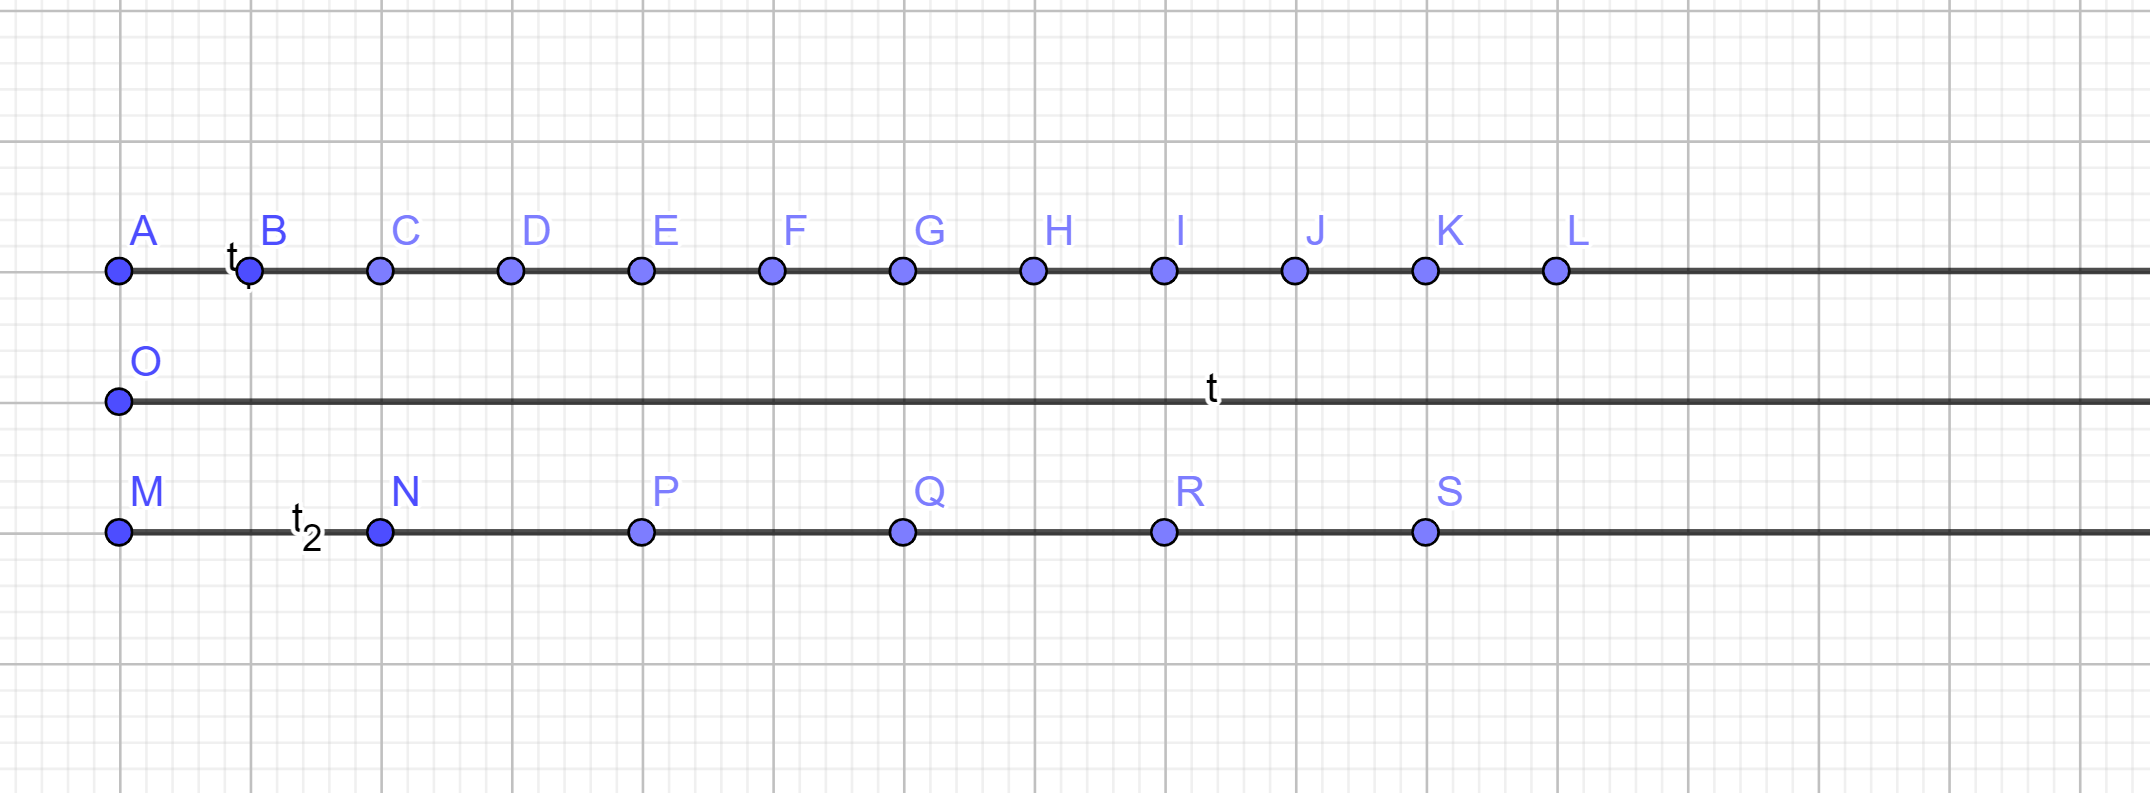
\includegraphics[width=1\textwidth]{Integrators/images/geogebra-export.png}
    \caption{Representation of how different forces with different timesteps are computed related to the actual flow of time.}
    \label{multiple_timestepping_img}
\end{figure}
At every step, I should compute the total force summing the value for the stiff component at each timestep and the most recent value for the soft component.
\begin{algorithm}[H]
            \caption{A first basic algorithm for the computation of multiple time stepping problems. Notice that, before entering the loop, we should recompute the forces and that the forceslow command is associated to soft springs while forcefast to stiffer.}
            \label{multiple_time_stepping_1}
			\begin{algorithmic}[1]
				\For{$i=1,...,nsteps$}
				\State $p=p+f*\Delta t/2$
				\State $q=q+p/m *\Delta t$
				\If{$i\% N == 0$}  
				    \State $f_S = forceslow(q)$ 
				\EndIf 
				\State $f_F = forcefast(q)$  
				\State $f = f_F + f_S$
				\State $p=p+f*\Delta t/2$	
				\EndFor
			\end{algorithmic}
\end{algorithm}
The main issue of this procedure is that this is not time reversible. If we start from the final point, the force at the i-th step is computed using a different value of the soft force at the nearest step. An algorithm that doesn't hold this reversibility, is not a good choice, as checking the energy conservation is not meaningful. To obtain reversible multiple time stepping, we should use a different path, exploiting Trotter-Splitting.\\
So, let's analyze this Hamiltonian,
\begin{equation}
    H = K + U_F + U_S
\end{equation}
where $U_F$ is the energy contribution given by stiffer springs and $U_S$ is the one given by softer springs plus some type of intermolecular interaction, which doesn't account tremendously on the energy of the system (Notice that non-interacting atoms could be removed from the simulation). In this situation, the Liouville operator $\widehat{L}$ is gonna be
\begin{equation*}
    \hat{L} = \hat{L}_q + \hat{L}_F + \hat{L}_S.
\end{equation*}
So,
\begin{equation}
    e^{-\hat{L}\Delta t} \simeq e^{-\frac{\hat{L}_S\Delta t}{2}} e^{-(\hat{L}_q + \hat{L}_F)\Delta t} e^{-\frac{\hat{L}_S\Delta t}{2}}.
\end{equation}
We can easily obtain the external terms, as they are just related to $\hat{L}_S$, while internal terms are not as easy because $[\hat{L}_q,\hat{L}_F] \neq 0$. So,
\begin{equation}
e^{-\frac{\hat{L}_S\Delta t}{2}} e^{-(\hat{L}_q + \hat{L}_F)\Delta t} e^{-\frac{\hat{L}_S\Delta t}{2}} = e^{-\frac{\hat{L}_S\Delta t}{2}} [e^{-(\hat{L}_q + \hat{L}_F)\frac{\Delta t}{N}}]^{N} e^{-\frac{\hat{L}_S\Delta t}{2}}.
\end{equation}
where N has a very important interpretation: in fact, it is the number of steps needed to make before recomputing $f_S$. In particular, it is related to the error I'm accepting in the inner parentheses: the bigger it is, the lower the error accepted and, clearly, the more expensive my calculations. Now, we can apply again the Trotter-Splitting for a shorter timestep, as the fast force changes very quickly.
\begin{align}
 e^{-\frac{\hat{L}_S\Delta t}{2}} [e^{-(\hat{L}_q + \hat{L}_F)\frac{\Delta t}{N}}]^{N} e^{-\frac{\hat{L}_S\Delta t}{2}} \simeq  e^{-\frac{\hat{L}_S\Delta t}{2}} [e^{-\hat{L}_F\frac{\Delta t}{2N}} e^{-\hat{L}_q\frac{\Delta t}{N}} e^{-\hat{L}_F\frac{\Delta t}{2N}}]^{N} e^{-\frac{\hat{L}_S\Delta t}{2}}.
\end{align}
Notice that the approximation made because of Trotter-Splitting is very refined because of the very short step assumed.\\
At this point what is important is to set our main timestep. From what we just saw, we have two possible choices, $\delta t = \frac{\Delta t}{N}$ or $\Delta t = \delta t *N$, where we respectively fix $\Delta t$ (the outer-parentheses timestep) and $\delta t$ (the inner-parentheses timestep). The first choice corresponds to a more accurate implementation while the second is faster. Assuming, for now, the first formulation, we can implement our code in the following way :
\begin{algorithm}[H]
            \caption{An algorithm based on Trotter Splitting and obtained by fixing $\Delta t$.}
            \label{multiple_time_stepping_2}
			\begin{algorithmic}[1]
				\For{$i=1,...,nsteps$}
				\State $p+=f_S*\Delta t/2$
				\For{$j=1,...,N$}
				    \State$p+=f_F*\frac{\Delta t}{2*N}$
				    \State$q+=\frac{p}{m}*\frac{\Delta t}{N}$
				    \State$f_F=forcefast(q)$
				    \State$p+=f_F*\frac{\Delta t}{2*N}$
				\EndFor
				\State $f_S=forceslow(q)$
				\State $p+= f_S * \frac{\Delta t}{2}$
				\EndFor
			\end{algorithmic}
\end{algorithm}
The other way to implement this algorithm (by fixing the $\delta t$ and changing the value of $\Delta t$ consequently) is produced by getting rid of one of the loops of Alg.\ref{multiple_time_stepping_2}, such that the new code would be
\begin{algorithm}[H]
            \caption{An algorithm based on Trotter Splitting and obtained by fixing $\delta t$.}
            \label{multiple_time_stepping_3}
			\begin{algorithmic}[1]
				\For{$i=1,...,nsteps$}
				\State $p+=f_F*\delta t/2$
			    \If{$istep \% N==0$}
			    \State $p+= f_S*\frac{\Delta t}{2}$
			    \EndIf
			    \State$q+=\frac{p}{m}*\delta t$
			    \State$f_F=forcefast(q)$
			    \State$p+=f_F*\frac{\delta t}{2}$
			    \If{$istep \% N == 0$}
			    \State$f_S=forceslow(q)$
			    \State$p+=f_S*\frac{\Delta t}{2}$
			    \EndIf
				\EndFor
			\end{algorithmic}
\end{algorithm}
Notice that in Alg.\ref{multiple_time_stepping_3} we substituted the outer loop of the two in Alg.\ref{multiple_time_stepping_2} with an if statement that detects which iteration of the inner loop corresponds to an iteration of the outer too. This way makes the code more practical and faster especially because of the cost of the calculations of $f_S$. But there is also a deeper reason. This second method makes it easy to compute a situation with a generic number of forces with different timesteps, as it consists only in adding new if statements instead of loops (which would slow down the code). The only parameter to be aware of is the $\Delta t$, which has to be adjusted coherently with the number of steps we want to wait for each force. A physical interpretation would be that we don't apply a force instantly every step nonetheless the amount of momentum we want to transfer is the same, so, since we apply forces later, we multiply them by a factor that makes the transfer identical.\\
How can we estimate N? Theoretically, we should estimate it through the ratio of the stiffness of the springs, but truly we try different values and look for the one which returns us energy conservation. We use a similar approach for estimating the timestep practically, but theoretically, saying we know the period of the stiffer springs, we should choose it smaller than $\frac{T}{\pi}$ for these last ones, while for the softer ones we should choose a limit value proportional to this period according to the ratio of the stiffness of the two types of springs, such that
\begin{equation*}
    \delta t < \frac{T}{\pi}=t_{limit}, \qquad \Delta t < t_{limit}*\frac{k_F}{k_S},
\end{equation*}
where $k_F$ and $k_S$ are the stiffness coefficient of the springs.\\
Moreover, this algorithm is time-reversible (both in the faster and in the accurate case). How can we see it ? Let's take a look at the order which we are applying to the operators. When we reverse it, we apply firstly the outer-parentheses operators which is exactly identical in both ways and then the inner-parentheses ones, which again has symmetrical form. In a more formal way, the Trotter Splitting method is time reversible and each individual block is time reversible as they correspond to Hamilton equations of fictitious systems. Because of this last property, this algorithm also preserves the volume in the phase space. It's important to notice that what we just did for the potential energy can be translated to the kinetic energy too if we have particles with masses very different between each other (it's usually applied to decomposed potential energy).
\subsection{Application}
Let's analyze a real case application of multiple timestepping. We have a system of biatomic molecules which interact with each other via the Lennard-Jones potential. The potential energy will be 
\begin{equation}
    U = U_{springs} + U_{LJ}^{short-range} + U_{LJ}^{long-range}
\end{equation}
where $U_{LJ}^{short-range} + U_{LJ}^{long-range}$ account for the entire Lennard-Jones potential. The "fast" component is gonna be $U_{springs} + U_{LJ}^{short-range}$ while the "slow" one is gonna be $U_{LJ}^{long-range}$.
\begin{figure}[h]
    \centering
    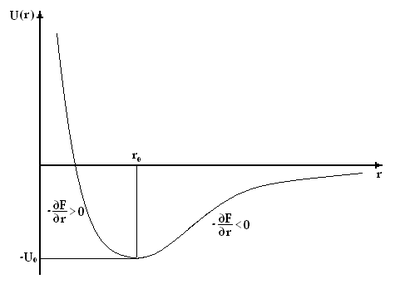
\includegraphics[width=0.70\textwidth]{Integrators/images/Lennard-Jones.png}
    \caption{The Lennard-Jones potential. We divide it into two components, a short-range one and a long-range one.}
    \label{Lennard-Jones}
\end{figure}
In this case, the multiple timestepping method makes sense to be used as long as we consider that most of the molecules stay far from each other, so that the Short-Range (S-R) interaction is less frequent compared to the Long-Range (L-R) ones, which will be, consequently, more expensive to compute as most of the molecules are far from each other. How do I know a priori which pair of particles are close to each other if they can move from their starting position ? I exploit a particular computational artifice called the neighbour list. Without going too much in depth into this specific topic, let's just understand that this is a typical application of multiple timestepping, where S-R forces have short time steps and L-R ones have longer time steps. What matters, at the end of the day, is not only how stiff the spring is but also how fast the atoms will move, so their mass too.\\
What happens if we want to compute a potential in the most accurate way possible ? We could consider having a very accurate yet expensive way to compute forces and, on the side, a force field like L-J. What we could do is rewriting our potential energy as
\begin{equation}
    U = U_{FF} + (U_{ACC} - U_{FF}).
\end{equation}
where $U_{ACC}$ and $U_{FF}$ are respectively the accurate and the simple potentials.
If the term $U_{ACC} - U_{FF}$ is small, we could calculate the two parts at different time steps (the first for short steps and the second for larger steps).\footnote{If you are interested on this topic, check the following paper :M. Tuckerman, B. J. Berne, and G. J. Martyna "Reversible Multiple Time Scale Molecular Dynamics" https://doi.org/10.1063/1.46313797}